\documentclass[a4paper, 11pt]{report}

\usepackage{array}
\usepackage{textcomp}
\usepackage{geometry}
\usepackage{todonotes}
\usepackage{makeidx}
\usepackage{mdframed}
\usepackage{listings}
\graphicspath{{Schemas/}}

\definecolor{light-gray}{gray}{0.95} %the shade of grey that stack exchange uses
\lstset{
  literate=
  {á}{{\'a}}1 {é}{{\'e}}1 {í}{{\'i}}1 {ó}{{\'o}}1 {ú}{{\'u}}1
  {Á}{{\'A}}1 {É}{{\'E}}1 {Í}{{\'I}}1 {Ó}{{\'O}}1 {Ú}{{\'U}}1
  {à}{{\`a}}1 {è}{{\`e}}1 {ì}{{\`i}}1 {ò}{{\`o}}1 {ù}{{\`u}}1
  {À}{{\`A}}1 {È}{{\'E}}1 {Ì}{{\`I}}1 {Ò}{{\`O}}1 {Ù}{{\`U}}1
  {ä}{{\"a}}1 {ë}{{\"e}}1 {ï}{{\"i}}1 {ö}{{\"o}}1 {ü}{{\"u}}1
  {Ä}{{\"A}}1 {Ë}{{\"E}}1 {Ï}{{\"I}}1 {Ö}{{\"O}}1 {Ü}{{\"U}}1
  {â}{{\^a}}1 {ê}{{\^e}}1 {î}{{\^i}}1 {ô}{{\^o}}1 {û}{{\^u}}1
  {Â}{{\^A}}1 {Ê}{{\^E}}1 {Î}{{\^I}}1 {Ô}{{\^O}}1 {Û}{{\^U}}1
  {œ}{{\oe}}1 {Œ}{{\OE}}1 {æ}{{\ae}}1 {Æ}{{\AE}}1 {ß}{{\ss}}1
  {ű}{{\H{u}}}1 {Ű}{{\H{U}}}1 {ő}{{\H{o}}}1 {Ő}{{\H{O}}}1
  {ç}{{\c c}}1 {Ç}{{\c C}}1 {ø}{{\o}}1 {å}{{\r a}}1 {Å}{{\r A}}1
  {€}{{\EUR}}1 {£}{{\pounds}}1,
  numbers=left,
  numbersep=10pt,
  showspaces=false,
  showstringspaces=false,
  showtabs=false,
  stepnumber=1,
  stringstyle=\color{gray},
  tabsize=4,
  basicstyle=\small,
  keywordstyle=\bf\color{blue},
  backgroundcolor=\color{light-gray},
  commentstyle=\color{ForestGreen},
  showstringspaces=false
}
\geometry{hmargin=2cm, vmargin=2cm}

\begin{document}

\chapter{Matériel}
\section{Machine virtuelle}
	\subsection{Environnement de travail}
		Cette partie explique les intstallations effectuées sur la machine virtuelle, nous détaillerons plus tard le choix des programmes installés.
		Pour travailler sur la machine virtuelle, nous nous sommes connectés en \emph{ssh}.
		\subsubsection{Système d'exploitation}
			Le système d'exploitation de la machine virtuelle est \emph{CentOS}, pour le savoir il suffit de lire le contenu du fichier \emph{/proc/version}.
			Dans notre cas, il contient : 
			\begin{mdframed}[backgroundcolor=light-gray, roundcorner=20pt,
				leftmargin=0, rightmargin=0, 
				innerleftmargin=20, linecolor=darkgray]
				Linux version 3.10.0-1062.4.3.el7.x86\_64 (mockbuild\@kbuilder.bsys.centos.org) (gcc version 4.8.5 20150623 (Red Hat 4.8.5-39) (GCC) ) \#1 SMP Wed Nov 13 23:58:53 UTC 2019
			\end{mdframed}
			Cette information nous permettra de savoir comment installer les programmes dont nous auront besoin.
		\subsubsection{Installation des logicielles}
			Pour installer un programme, on peut utiliser le gestionnaire de paquets de CentOS : \emph{yum}.
			Il faudra ensuite lancer les commandes suivantes, qui installent respectivement Java, le \emph{Système de Gestion de Base de Données}, screen, netcat, nmap
			\begin{mdframed}[backgroundcolor=light-gray, roundcorner=20pt,
				leftmargin=0, rightmargin=0, 
				innerleftmargin=20, linecolor=darkgray]
				\begin{lstlisting}[language=bash]
					sudo yum install java-1.8.0-openjdk
					sudo yum install mysql-server
					sudo yum install screen
					sudo yum install nc
					sudo yum install nmap
				\end{lstlisting}
			\end{mdframed}
		\subsubsection{Paramétrage du SGBD}
\chapter{Choix BDD}
\section{Base de données}
\subsection{Choix de la base de donnée}
	Nous avons tout d'abord dû choisir quelle technologie nous allions utilisé pour notre base de données.
	Nous connaissions en connaissions un nombre suffisant pour ne pas chercher autre chose et juste faire un choix.
	\par
	\begin{center}
		Technologies que nous connaissions
		\par
		\begin{tabular}{|l|c|c|c|c|}
			\hline
			Nom & Niveau de connaissance & Facilité d'intégration & License \\
			\hline
			PostGreSQL & Inconnu & Oui & Oui\\
			\hline
			MySQL & Bon & Oui & Oui & GPLv2\\
			\hline
			Oracle Database & Bon & Oui & Oui \\
			\hline
			sqlite3 & Bon & Non & Oui \\
			\hline
		\end{tabular}
	\end{center}
\section{Communication avec l'application}
\subsection{Serveur}
\subsection{Protocole}
	\begin{center}
		Liste des messages possibles dans le sens clients $\rightarrow$ serveur
		\par
		\begin{tabular}{|l|l|}
			\hline
			Commande & Utilisation\\
			\hline
			Subscribe:$<id>:<mdp>$ & Permet de s'inscrire\\
			\hline
			Connect:$<id>:<mdp>$ & Permet de se connecter à son compte\\
			\hline
			\hline
			History:$<debut>:<fin>$ & Permet de récupérer $x$ trajets entre début et fin (en id)\\
			\hline
			Projects:$<debut>:<fin>$ & Permet de récupérer les $x$ projets entre début et fin\\
			\hline
			\hline
			NewP:$<nom>:<x+y+z;...>$ & Ajoute un nouveau projet\\
			\hline
			NewJ:$<nom>:<x+y+z+t;...>$ & Ajoute un nouveau trajet\\
			\hline
			EditP:$<id>:<x+y+z;...>$ & Modifie un projet\\
			\hline
		\end{tabular}
	\end{center}
	\begin{center}
		Liste des messages possibles dans le sens serveur $\rightarrow$ client
		\par
		\begin{tabular}{|l|l|}
			\hline
			Commande & Utilisation\\
			\hline
			Subscribed:$<id>$ & Confirme l'inscription \\
			\hline
			Unsubscribed & Erreur lors de l'inscripton \\
			\hline
			Connected:$<id>$ & Valide la connection à son compte\\
			\hline
			Unconnected & Erreur lors de la connection \\
			\hline
			\hline
			Project:$<id>:<nom>:<x+y+z;...;x+y+z>$ & Envoie des informations sur un projet\\
			\hline
			Journey:$<id>:<nom>:<d>:<x+y+z+t...>$ & Envoie des informations sur un projet\\
			\hline
		\end{tabular}
	\end{center}
\chapter{Serveur}
\section{Architecture}
	\subsection{Processus}
		Le serveur utilise une architecture avec plusieurs processus. Le processus principal attend une connection provenant d'un client (application).
		A chaque connection un nouveau processus est créé pour intéragir avec le client. Ce processus attend donc un message du client, exécute la commande
		SQL nécessaire pour obtenir une réponse et enfin, il répond au client en formattant les données. Un processus supplémentaire existe pour pouvoir
		travailler directement avec le serveur, sans passer par un client. Pour cela, l'entrée et la sortie standard sont utilisées et il faut donc un accès direct à la machine.
	\subsection{Classes}
		Le processus principal n'utilise qu'une seule classe \emph{Serveur}, tout comme le processus de communication direct \emph{LocalCommand}.
		Cependant le processus de communication avec le client est séparé en plusieurs objets : \emph{Client}, \emph{SQLHandler} et \emph{CommunicationHandler}. 
		Le premier est le processus en lui même et utilise les deux autres pour effectuer les tâches qui lui sont assignées. L'objet \emph{SQLHandler} accède à la base de données et formatte les réponses.
		Enfin le \emph{CommunicationHandler} gère la communication réseau avec le client, il permet la réception et l'envoie de chaîne de caractères.
		Enfin deux classes sont utilisées pour facilité le travail de conversion des formats pour les points : \emph{Point3D} et \emph{Point4D} qui correspondent respectivement à une coordonnée dans l'espace : (x, y, z)
		et à une coordonnée dans l'espace et le temps : (x, y, z, t).
	\subsection{Echange type}
		TODO : Diagramme de séquence
\section{Implémentation}
	\subsection{Langage}
		La création du serveur devait à l'origine être rapide car on le considérait comme étant annexe. C'est pourquoi on a choisi l'utilisation d'une
		technologie que nous connaissions déjà : \emph{Java}. Ce langage contient dans sa librairie standard tout ce qu'il faut pour développer un serveur.
		De plus il existe une librairie java développée par Oracle pour la communication avec les bases de données MySQL.
		\subsubsection{Machine Virtuelle}
			Le \emph{Java} est un langage compilé particulier. Le code est tout d'abord compilé dans un langage intermédiaire appelé \emph{Bytecode}. 
			Puis, il est exécuté dans une machine virtuelle appelée la \emph {Java Virtual Machine} en utilisant une nouvelle étape de compilation \emph {Just In Time}.
			\par
			\begin{center}
				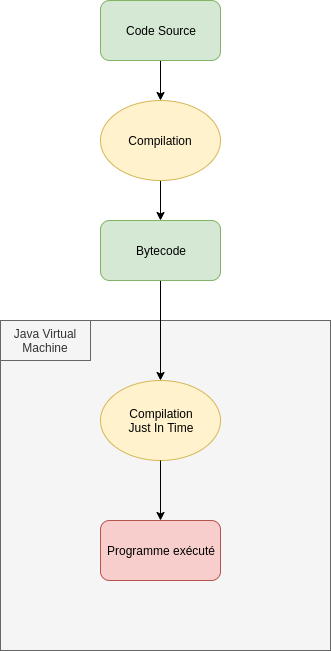
\includegraphics[scale=0.5]{java_compilation.png}
			\end{center}
			Les programmes développés et compilés en Java peuvent être exécuté sur toutes les machines possédant la JVM installée sans avoir aucun changement de code source ou bien de paramêtre de compulation.
	\subsection{Fonctionnement des processus}
		L'organisation des processus en java est particulière. En effet, il n'y a qu'un seul processus lourd (à la différence des forks du langage C).
		Ce processus lourd unique est la JVM. Tous les autres processus, y compris le processus principal de notre programme ne sont que des processus légers.
		Il y a donc un partage des resources, et l'échange de données est plus simple. Il faut attention faire cependant aux accès simultanés aux ressources.
		\subsubsection{Création de processus}
			Le processus principal de notre programme est créé automatiquement par la JVM et il exécute le code de la fonction \emph{public static void main(String[] args)} qui est le point d'entrée de notre programme.
			Pour construire d'autres processus il y a plusieurs manières. On va ici se concentrer sur la classe \emph{Thread} et l'interface \emph{Runnable}.
		\subsubsection{Utilisation de \emph{Thread}}
			Un \emph{Thread} est un objet qui exécute du code dans un autre processus. Pour cela, il suffit de créer un Thread et de le lancer en utilisant la méthode \emph{start()}.
			\begin{mdframed}[backgroundcolor=light-gray, roundcorner=20pt,
				leftmargin=0, rightmargin=0, 
				innerleftmargin=20, linecolor=darkgray]
				\begin{lstlisting}[language=Java]
					Thread monThread = new Thread();
					monThread.start();
				\end{lstlisting}
			\end{mdframed}
			Pour changer le code exécuté, il suffit de redéfinir la méthode \emph{void run()} de Thread.
			 \begin{mdframed}[backgroundcolor=light-gray, roundcorner=20pt,
				leftmargin=0, rightmargin=0, 
				innerleftmargin=20, linecolor=darkgray]
				\begin{lstlisting}[language=Java]
					Thread monThread = new Thread() {
						@Override
						public void run() {
							System.out.println("Dans un nouveau processus");
						}
					}
					monThread.start();
				\end{lstlisting}
			\end{mdframed}
	\subsection{Patron de conception}
		TODO : Fabric/Builder sur le serveur pour les clients\\
		TODO : Singleton Serveur + (LocalCommand ???)
	\subsection{Communication réseau}
		TODO : Expliquer Serveur Socket et Socket, le accept()\\
		TODO : Insérer le protocole de communication écrit plus haut
\chapter{Problèmes rencontrés}
\section{VPN}
	TODO: Problème de connexion au Téléphone
\section{VM}
	\todo{Règles du firewall}
	\todo{Machine éteinte !!!}
\end{document}

